% Chapter Template

\chapter{Placing into Context} % Main chapter title

\label{Chapter3} % Change X to a consecutive number; for referencing this chapter elsewhere, use \ref{ChapterX}

\lhead{Chapter 3. \emph{Placing into Context}} % Change X to a consecutive number; this is for the header on each page - perhaps a shortened title

%----------------------------------------------------------------------------------------
%	SECTION 1
%----------------------------------------------------------------------------------------

\section{Automotive industry}

The term automotive was created from Greek autos (self), and Latin motivus (of motion) to represent any form of self-powered vehicle.

It represents all those companies and activities involved in the manufacture of motor vehicles, including most components, such as engines and bodies. It is one of the world's most important economic sectors by revenue. The automotive industry does not include industries dedicated to the maintenance of automobiles following delivery to the end-user, such as automobile repair shops and motor fuel filling stations.

By allowing consumers to commute long distances for work, shopping, and entertainment, the auto industry has encouraged the development of an extensive road system, made possible the growth of suburbs and shopping centers around major cities, and played a key role in the growth of ancillary industries, such as the oil and travel businesses. The auto industry has become one of the largest purchasers of many key industrial products, such as steel. The large number of people the industry employs has made it a key determinant of economic growth.

\section{Car Diagnostic}
Performing a car diagnostic can reveal a number of problems associated with the transmission, oil tank, gas tank, exhaust system and other components of the vehicle. Modern vehicles designed with computer processors, microchips and sensors can be linked to a car diagnostic computer scan to pinpoint exactly where the problem exists. The scans are performed at a dealership or at the garage of certified mechanic. Some scans can be performed at home using a hand-held scanning device.

\subsubsection{History}
According to popularmechanics.com, in 1996 the EPA mandated that the computer interface of all vehicles sold in the United States had to meet the On-Board Diagnostics, version II (OBD II) standard. This meant that aftermarket repair shops would be able to diagnose a problem in the vehicle using only one set of tools and running a simple computer scan. This is now known as the car diagnostic test; the process involves producing a complete report with a set of codes that pertain to different problems.
\subsubsection{Effects}
The car diagnostic can tell you the following about the vehicle: ignition timing issues, level of buildup in the combustion engine, fuel injector performance, whether the ignition coils are firing, engine rpm levels, air and coolant temperature, crankshaft and camshaft position and the throttle opening. After the car diagnostic is performed, the computer will tag each data point to reveal what needs to be corrected and stores this code so that the technician can look in a specific area for the problem.

\subsubsection{Common Diagnostic Codes}
According to Car2Pro.com, OBD II diagnostic trouble codes can range from P0100 to P1899. Each letter and number in the code represents a different part of the vehicle. The first letter is often a "P," which relates to the powertrain. If it is a "B," it will relate to the body, a "C" relates to the chassis and a "U" is undefined.

The number zero in the second placeholder is a generic code shared by all manufacturers, but some manufacturers use a specific code here so the number 1 may appear. The third placeholder determines the area of the problem. A 1 means there is a fuel or air problem; 2 means there is something wrong with the injector circuit; 3 means there is an ignition problem or the engine is misfiring; 4 means there is an emission control problem; 5 means there is a vehicle speed or idle control problem; 6 means there is a computer or output circuit problem; a 7 or an 8 means there is a transmission problem. The fourth and fifth digits of the computer diagnostic check report further identify which system is malfunctioning; the digits that appear here vary by vehicle make, so the mechanic running the test may need to contact the dealership or do some research on what the rest of the code means.
\begin{figure}[h!]
  \centering
    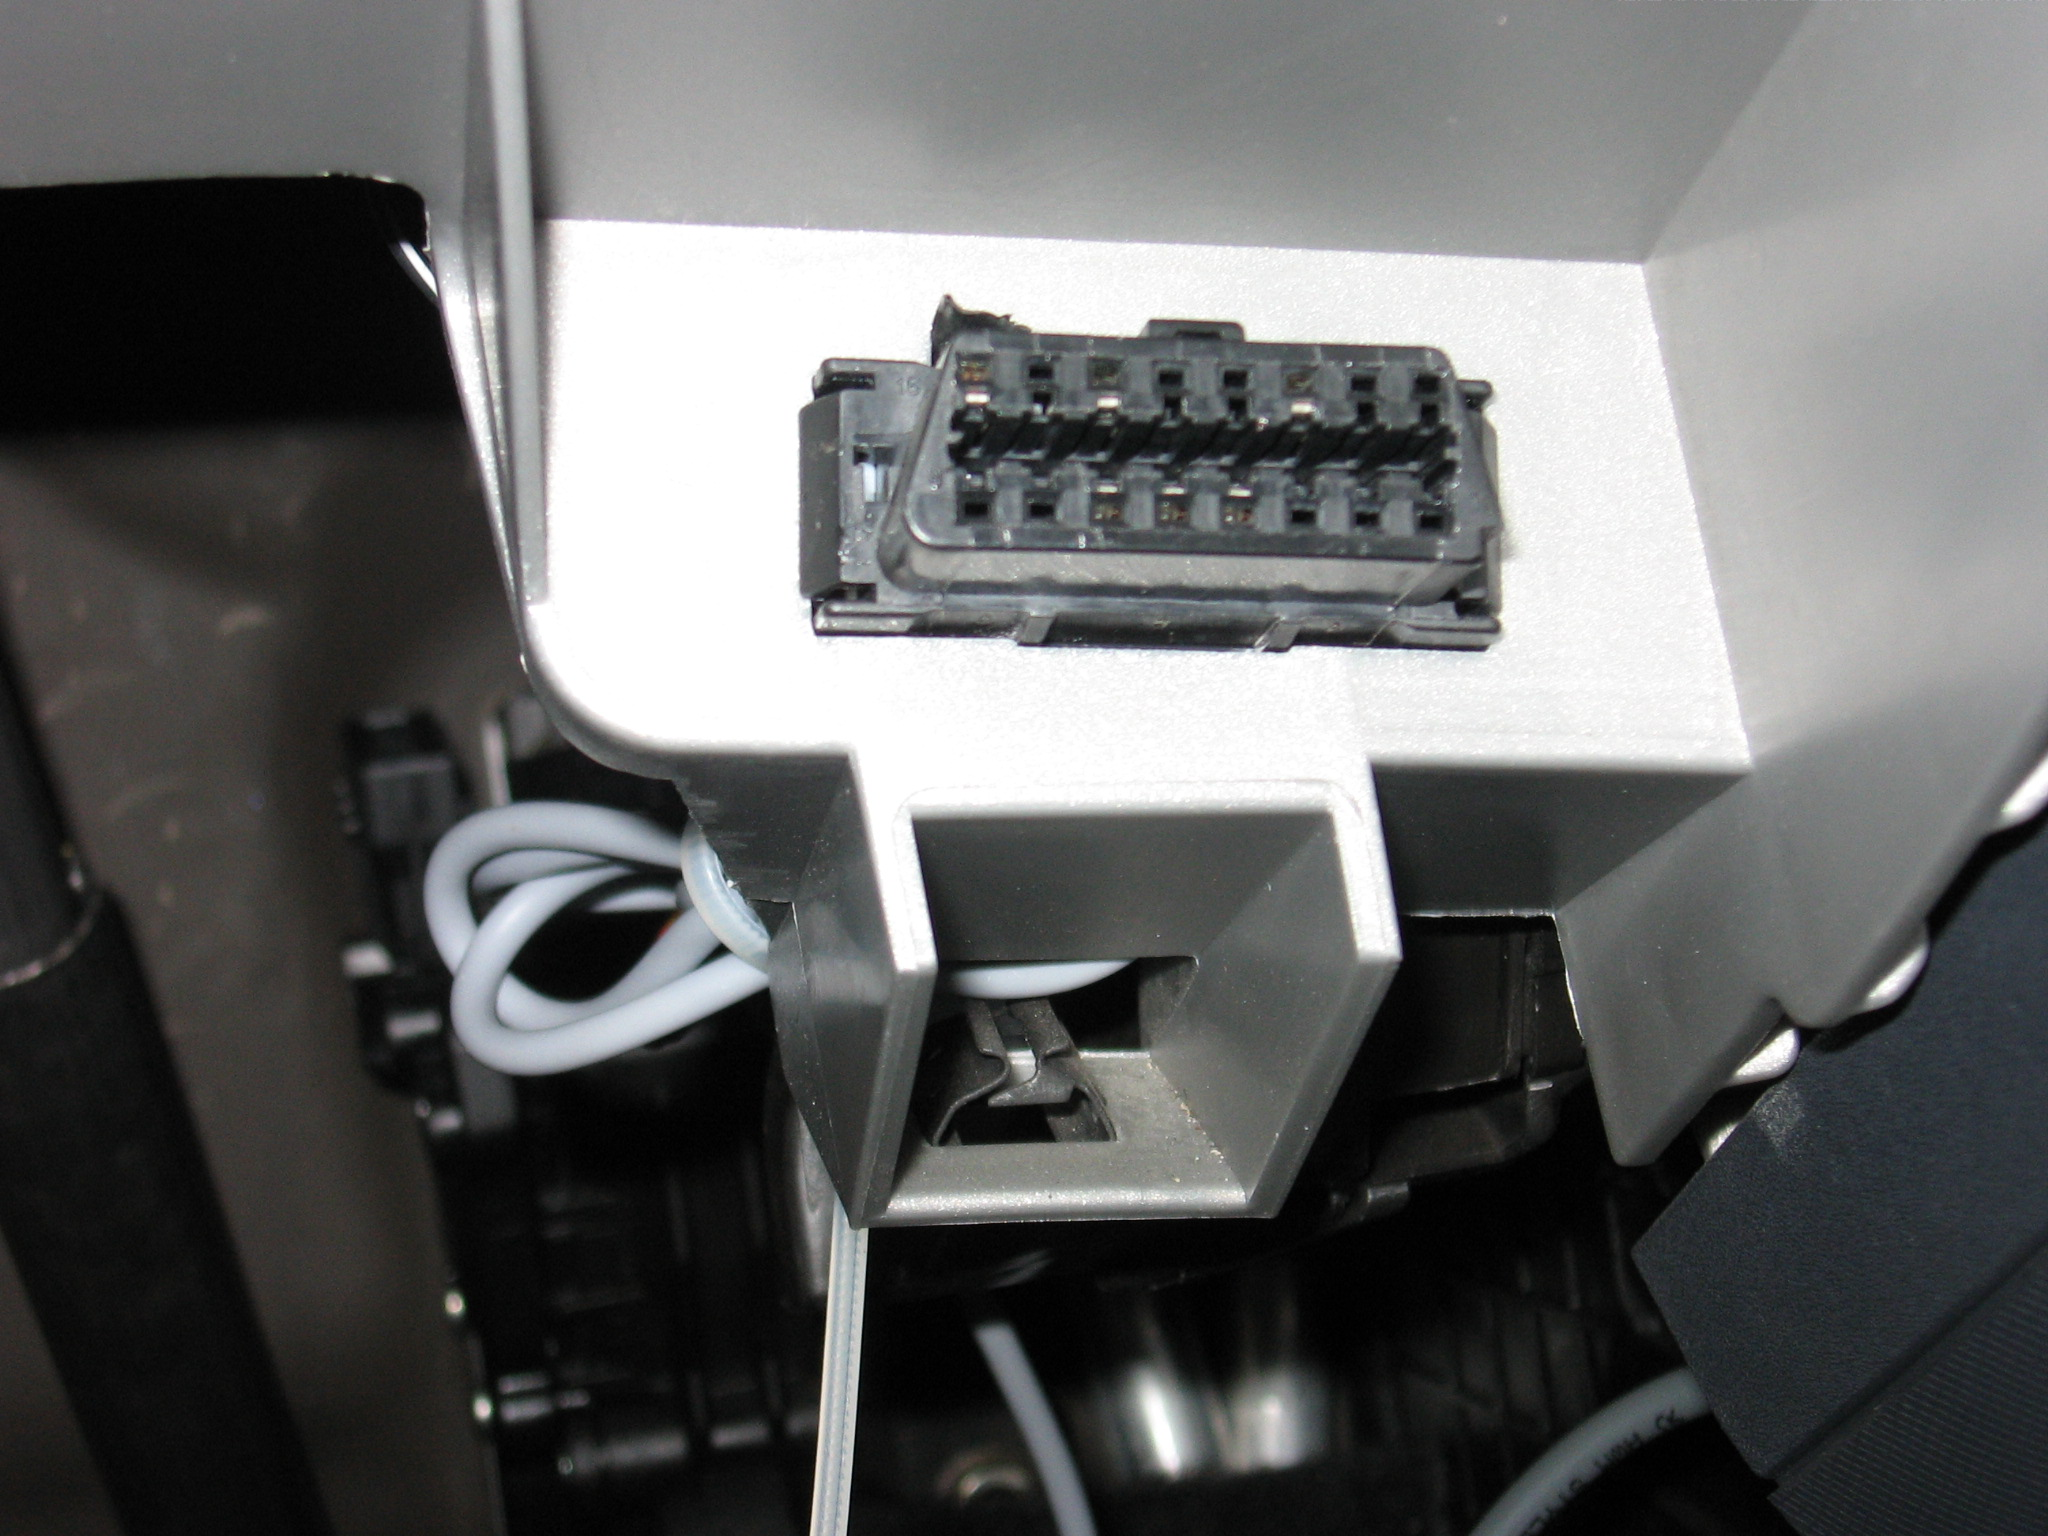
\includegraphics[width=1\textwidth]{./Pictures/OBD_002.jpg}
  \rule{1\textwidth}{1pt}
 \caption{Female OBD-II connector on a car}
\end{figure}

\paragraph*{On-board diagnostics}
\hfill \break
On-board diagnostics (OBD) is an automotive term referring to a vehicle's self-diagnostic and reporting capability. OBD systems give the vehicle owner or repair technician access to the status of the various vehicle subsystems. The amount of diagnostic information available via OBD has varied widely since its introduction in the early 1980s versions of on-board vehicle computers. Early versions of OBD would simply illuminate a malfunction indicator light or "idiot light" if a problem was detected but would not provide any information as to the nature of the problem. Modern OBD implementations use a standardized digital communications port to provide real-time data in addition to a standardized series of diagnostic trouble codes, or DTCs, which allow one to rapidly identify and remedy malfunctions within the vehicle.

\subsubsection{Costs}
The price of an average car diagnostic can range from \$20 to \$400 depending on the type of scanner used and the make and model of the vehicle, according to popularmechanics.com. Consumer code readers are available, but these only provide limited information on the source of the problem.

\subsubsection{Benefits}
Performing a car diagnostic test using an auto scan tool can save the mechanic a lot of time troubleshooting a problem and also save the car owner money because they don't have to pay for a complete mechanical check at their local repair shop. When the "Check Engine" light appears in the dashboard, the car owner has no idea what could be causing the problem. Running a computerized car diagnostic check can highlight the problem so that the mechanic can fix only what needs to be fixed. Most car diagnostic checks can be performed in under an hour.



